% Виды параметризации прямых на изображении и их свойства. Повторное вычисление преобразования Хафа и связь этой процедуры с поиском точки схода.

Количество прямых на дискретном изображении размера $n \times n$ можно оценить как $\Theta\left( n^2 \right)$, хотя точное количество зависит от выбранной параметризации. Обычно рассматривают следующие способы:
\begin{itemize}
\item
    $\left( \rho, \phi \right)$-параметризация. Прямая, описанная такими параметрами, принадлежит к семейству параллельных прямых, направляющий вектор которых имеет угол $\phi$, а расстояние от начала координат до этой прямой равно $\rho$. Таким образом, ортогональная проекция начала координат на эту прямую в полярных координатах имеет координаты $\left( \phi + \frac{\pi}{2}, \rho \right)$.

    Преобразование построенной непрерывной прямой в дискретную обычно делается при помощи алгоритма Брезенхема. Для преимущественно горизонтальных прямых ($\left|\frac{dy}{dx}\right| \le 1$) в каждом столбце выбирается один пиксель, центр которого ближе всего к пересечению прямой с соответствующей вертикалью. Если прямая -- преимущественно вертикальная, то используется аналогичная стратегия с заменой строк на столбцы и наоборот.

    Такая параметризация ограничена, поскольку $\phi$ изменяется от $0$ до $\pi$, а $\rho$ -- от $-\frac{n}{\sqrt{2}}$ до $+\frac{n}{\sqrt{2}}$ (или $\left[ 0, 2\pi \right)$ и $\left[ 0, \frac{n}{\sqrt{2}} \right]$ соответственно), но нелинейна, так как множество пар $(\rho, \phi)$, проходящих через заранее выбранную точку, образует не прямую, а синусоиду.
\item
    $\left( k, b \right)$-параметризация. Описывает непрерывную прямую, заданную уравнением $y=kx+b$. В этой параметризации из рассмотрения исключаются вертикальные прямые. Параметризация линейна, так как при фиксированных $(x, y)$ параметры $k, b$ связаны линейным соотношением, но не ограничена, поскольку $k$ будет принимать неограниченно большие значения для прямых, близких к вертикальным. Однако недостаток этой параметризации состоит в ее неравномерности: разница между $k=1$ и $k=2$ намного более значительна, чем между $k=100$ и $k=101$.

    Так же, как и в предыдущем пункте, дискретизация проводится при помощи алгоритма Брезенхема.
\item
    $\left( s, t \right)$-параметризация. Эта параметризация учитывает только преимущественно вертикальные прямые с наклоном вправо ($\frac{dx}{dy} \in \left[ 0, 1 \right]$). Прямая, соответствующая паре параметров $(s, t)$, проходит через середины пикселей с координатами $(s, 0)$ и $(s + t, n-1)$. Так как оба параметра изменяются от $0$ до $n-1$, второй пиксель в этой паре может выходить за пределы изображения, но это не должно быть проблемой, поскольку сетку координат всегда можно продлить. Дискретизация выполняется либо при помощи алгоритма Брезенхема, либо при помощи диадических паттернов.

    Такая параметризация является ограниченной, что было отмечено раньше, и линейной, так как точка $x, y$ принадлежит описыванной прямой, если выполняется следующее условие:
    \begin{gather}
    \label{5_1}
        x =
        s \cdot \left( \frac{y}{n-1} \right) + \left( s+t \right) \cdot \left( 1 - \frac{y}{n-1} \right) =
        s + t \cdot \frac{y}{n-1}, \\
    \nonumber
        s = \frac{y}{n-1} t - x.
    \end{gather}
\end{itemize}

Поскольку быстрое преобразование Хафа использует $(s, t)$-параметризацию, которая является линейной, то на Хаф-образе пучка прямых, проходящих через одну точку, заметна выделяющаяся прямая, то есть прямая с экстремально высокой суммой значений по содержащимся пикселям. Найдя параметры этой прямой, при помощи уравнения \eqref{5_1} можно определить точку пересечения пучка. Прямую с таким свойством можно найти, если еще раз применить к линограмме преобразование Хафа.

Следует отметить, что на настоящем изображении, на котором нужно выделить точку схода, после выделения границ будет множество шумовых линий, но все же большое количество линий проходит через одну точку, поэтому описанный алгоритм потенциально можно использовать. Рассмотрим условный искусственный пример.

На изображении \ref{img5_1} приведен пучок прямых, имитирующий линии разметки, проходящие через точку схода.

\begin{figure}[!h]
    \centering
    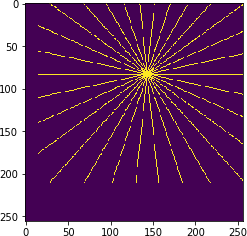
\includegraphics[width=0.3\linewidth]{5_1}
    \caption{Пучок прямых на изображении размера $256 \times 256$}
    \label{img5_1}
\end{figure}

На линограмме этого изображения \ref{img5_2} видно четыре яркие точки, соответствующие тем прямым, которые обладают нужным наклоном и могут быть определены при помощи БПХ. При этом эти точки лежат на одной прямой, поскольку соответствующие прямые пересекаются.

\begin{figure}[!h]
    \centering
    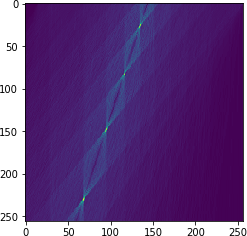
\includegraphics[width=0.3\linewidth]{5_2}
    \caption{Линограмма изображения \ref{img5_1}}
    \label{img5_2}
\end{figure}

Поскольку эта прямая имеет неправильный наклон, применим преобразование Хафа к линограмме, предварительно отразив ее по вертикали. На полученной линограмме \ref{img5_3} заметна одна яркая точка, соответствующая целевой точке схода, и четыре прямых, соответствующих некоторым прямым из исходного пучка. Однако координаты точки не соответствуют исходным и требуют пересчета в соответствии с \eqref{5_1}.

\begin{figure}[!h]
    \centering
    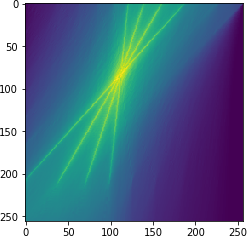
\includegraphics[width=0.3\linewidth]{5_3}
    \caption{Линограмма изображения \ref{img5_2}}
    \label{img5_3}
\end{figure}
